\section{Aufbau}
Der genutzte Versuchsaufbau ist in Abbildung $\ref{aufbau}$ dargestellt. Er besteht aus der, mit einer Heizwicklung umfassten, Kupferprobe, welche sich in einem Kupferzylinder befindet. Dieser verfügt ebenfalls über eine
separate Heizwicklung. Sowohl der Zylinder, als auch die Probe sind jeweils mit einem Pt-100 Wiederstand ausgestattet, welche als Thermometer dienen. Der Zylinder wird in einem Rezipienten befestigt, welcher an eine
Vakuumpumpe sowie eine Heliumquelle angeschlossen ist. Der Rezipient wird in ein mit flüssigem Stickstoff gefülltes Dewar-Gefäß gestellt.

\begin{figure}[H]
  \centering
  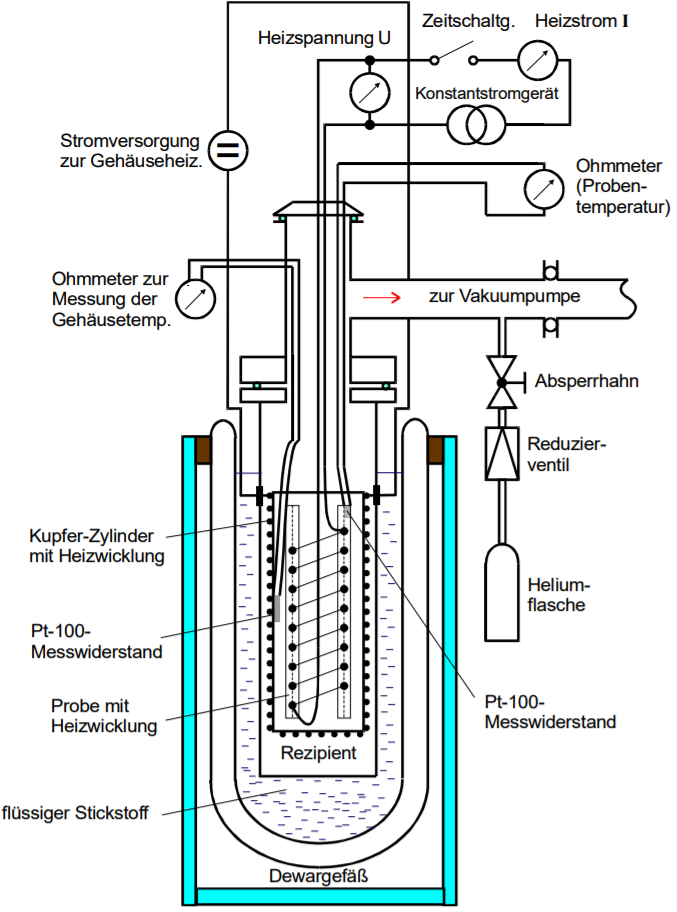
\includegraphics[width=0.5\textwidth]{Bilder/aufbau.png}
  \caption{Messrichtungen der Projektion.}
  \label{aufbau}
\end{figure}
\clearpage
Zur Untersuchung der Molwärme muss die Probe zunächst auf $\SI{80}{K}$ heruntergekühlt werden. Hierzu wird zunächst der Rezipient evakuiert und mit Helium als Wärmeleiter befüllt. Wenn die Zieltemparatur erreicht ist, wird das Helium wieder
abgepumpt. Die Heitzinstrumente von Probe und Zylinder werden eigenschaltet und es wird Heizspannung, Heizstrom, Heizdauer und Temperaturdifferenz in 7 bis 11 K schritten aufgezeichnet. Um Energieverluste durch
Wärmestrahlung zu vermeiden, werden Zylinder und Probe auf der gleichen Temperatur gehalten. Energieverluste durch Konvektion werden durch das Vakuum im Rezipienten verhindert.
